\chapter{MHealth System and Its Design Goals}
\label{Chapter4}

This chapter presents the architecture of the proposed mHealth system and the design goals that guided its development. The design goals were derived from a synthesis of the clinical literature, requirements analysis of the university counselling context, and feedback from a pilot study with students and counsellors. The system is implemented as a set of microservices that together implement the complete workflow from automated voice data collection to counsellor-facing depression risk reporting.

\section{Design Goals}

\subsection{DG1: Scalability}

The system must be capable of screening large numbers of students without requiring proportional increases in counsellor time. This necessitates automated data collection that runs without human intervention, and asynchronous backend processing that can handle concurrent calls and parallel ML inference.

\textit{Realisation}: The Twilio Voice API enables fully automated outbound calls once initiated. Celery workers process depression analysis asynchronously, decoupled from the call flow. Counsellors initiate calls to selected recipients directly from the Call Management dashboard — either individually or in bulk for multiple selected targets in a single action.

\subsection{DG2: Interpretability}

The system must produce outputs that counsellors can understand and evaluate. A binary prediction alone is insufficient; practitioners must be able to inspect the acoustic basis for a prediction to exercise informed clinical judgement~\cite{Thieme2020, Feng2024}.

\textit{Realisation}: The ML service returns not only a risk label and probability, but also per-segment probability distributions. Future iterations will integrate visualisations of key acoustic features (pitch variation, speaking rate, pause time, HNR, F0 statistics, jitter, shimmer) against reference distributions, enabling counsellors to see which vocal characteristics drove the prediction.

\subsection{DG3: Human-in-the-Loop}

The system must not replace clinical judgement. All predictions are advisory; the decision to contact a flagged student, conduct a formal assessment, or intervene rests entirely with the trained counsellor~\cite{Thieme2020}.

\textit{Realisation}: The counsellor dashboard presents depression risk as a probability score, not a diagnostic label. Counsellors review AI-flagged students through a dedicated ``Call recipients flagged by AI'' tab (shown in Figure~\ref{fig:ui_flagged}), where each flagged case displays the risk probability, call timestamp, and analysis score. No automated action is taken on the basis of the ML prediction — the counsellor always retains final authority.

\subsection{DG4: Privacy and Data Security}

Voice recordings and mental health assessments are highly sensitive personal data. The system must minimise external data exposure and handle recordings securely throughout their lifecycle.

\textit{Realisation}: Recordings are transferred from Twilio to a self-hosted MinIO object storage instance immediately after the call, minimising third-party data exposure. Presigned URLs with configurable expiry (default: 3,600 seconds) are used for time-limited playback. The PostgreSQL database stores no raw audio — only URLs and derived metadata. The dashboard is protected by JWT-based authentication with a secure login interface (Figure~\ref{fig:ui_login_cropped}).

\subsection{DG5: Non-Intrusiveness}

The data collection mechanism must minimise the psychological burden on participants and must not require them to install software, create accounts, or use unfamiliar devices~\cite{Maharjan2022}.

\textit{Realisation}: Twilio places outbound calls to students' personal mobile numbers. No app installation or account creation is required. Students respond verbally to questions over a standard phone call. The call script explicitly provides informed consent information at the outset.

\subsection{DG6: Integration with Counselling Workflows}

The system must fit into the existing operational context of a university counselling centre, providing outputs in formats that counsellors can act on within their existing workflows~\cite{Suendermann2019}.

\textit{Realisation}: The counsellor dashboard (Figure~\ref{fig:ui_about}) provides a single landing page with direct access to three operational modules: Twilio Call Management, Call Status Dashboard, and Admin Dashboard. All call records, audio playback, risk scores, and flagging history are aggregated in one interface.

\subsection{DG7: Continual Improvement}

The system should support the accumulation of labelled data in deployment, enabling periodic retraining of the ML model as institution-specific speech data grows.

\textit{Realisation}: Counsellor follow-up decisions (recorded via FlaggedTargets) serve as soft labels for retraining. The ML model is stored in a dedicated \texttt{model\_store} directory and can be replaced without service restart using lazy loading. All audio recordings are archived in MinIO and remain available for future retraining pipelines.

%-------------------------------------------------------------
\section{System Architecture}
%-------------------------------------------------------------

The system is implemented as a set of loosely coupled microservices communicating over HTTP and an asynchronous message queue. Figure~\ref{fig:system_arch} shows the high-level architecture. Table~\ref{tab:tech_stack} summarises the technology stack.

\begin{figure}[h]
\centering
\resizebox{\textwidth}{!}{%
\begin{tikzpicture}[
  svc/.style={rectangle, rounded corners=5pt, draw=black!70, minimum height=1.1cm,
              text width=3.0cm, align=center, font=\small},
  dbarrow/.style={-{Stealth[length=2.5mm]}, thick, draw=black!60},
  grp/.style={draw=black!35, dashed, rounded corners=6pt, inner sep=8pt},
  lbl/.style={font=\footnotesize\bfseries}
]
  % ---- Frontend ----
  \node[svc, fill=blue!12] (fe) at (0,0) {React Frontend\\(Counsellor Dashboard)};

  % ---- Backend ----
  \node[svc, fill=teal!12] (be) at (5.5,0) {FastAPI Backend\\(Orchestration / Auth)};

  % ---- Services row ----
  \node[svc, fill=green!12]  (ml)   at (1.5,-3.2) {ML Service\\(FastAPI, port 8001)};
  \node[svc, fill=purple!12] (twil) at (5.5,-3.2) {Twilio Voice API\\(IVR / TwiML)};
  \node[svc, fill=orange!12] (cely) at (9.5,-3.2) {Celery + RabbitMQ\\(Async Tasks)};

  % ---- Storage row ----
  \node[svc, fill=yellow!15] (pg)    at (3.5,-6.0) {PostgreSQL\\(Relational DB)};
  \node[svc, fill=gray!15]   (minio) at (7.5,-6.0) {MinIO\\(Object Storage)};

  % ---- Arrows ----
  \draw[dbarrow] (fe.east)  -- node[above,font=\tiny]{REST/HTTP} (be.west);

  \draw[dbarrow] (be.south) -- ++(0,-0.6) -| (ml.north);
  \draw[dbarrow] (be.south) -- ++(0,-0.6) -- (twil.north);
  \draw[dbarrow] (be.south) -- ++(0,-0.6) -| (cely.north);

  \draw[dbarrow] (be.south)  -- ++(0,-3.9) -| (pg.north);
  \draw[dbarrow] (cely.south)-- ++(0,-0.5) -| (minio.north);
  \draw[dbarrow] (twil.south)-- ++(0,-0.5) -| (minio.north);

  % ---- Group labels ----
  \begin{scope}[on background layer]
    \node[grp, fit=(ml)(twil)(cely), label={[lbl]above:Services}] {};
    \node[grp, fit=(pg)(minio),       label={[lbl]above:Storage}] {};
  \end{scope}
\end{tikzpicture}}
\caption{High-level microservices architecture of the proposed mHealth system. The React frontend communicates with the FastAPI backend, which orchestrates the ML service, Twilio IVR, and Celery task queue. Audio recordings are persisted in MinIO; metadata in PostgreSQL.}
\label{fig:system_arch}
\end{figure}

\begin{table}[h]
\centering
\caption{Technology stack for the proposed mHealth system.}
\label{tab:tech_stack}
\begin{tabular}{@{}lll@{}}
\toprule
\textbf{Component} & \textbf{Technology} & \textbf{Role} \\
\midrule
Frontend           & React (TypeScript), Vite, MUI & Counsellor dashboard \\
Backend API        & FastAPI (Python)               & Orchestration, routing, auth \\
ML Service         & FastAPI (Python)               & Depression inference \\
IVR / Call Service & Twilio Voice API + FastAPI     & Outbound calls, TwiML \\
Task Queue         & Celery + RabbitMQ             & Async archival and ML inference \\
Database           & PostgreSQL + SQLAlchemy        & Persistent storage \\
Object Storage     & MinIO                         & Audio recording archival \\
Migrations         & Alembic                       & Schema versioning \\
Authentication     & JWT                           & Admin access control \\
\bottomrule
\end{tabular}
\end{table}

%-------------------------------------------------------------
\section{Component Descriptions}
%-------------------------------------------------------------

\subsection{Frontend: Counsellor Dashboard}

The frontend is a React single-page application (SPA) built with TypeScript, Vite, and Material UI (MUI). It communicates with the backend exclusively via RESTful HTTP and provides a unified interface for all counsellor-facing operations.

\subsubsection{Authentication}

Access to the dashboard is controlled by JWT-based authentication. Figure~\ref{fig:ui_login} shows the login screen, which supports both direct email/password login and institute single sign-on via INAS (Institute Authentication Services).

\begin{figure}[h]
    \centering
    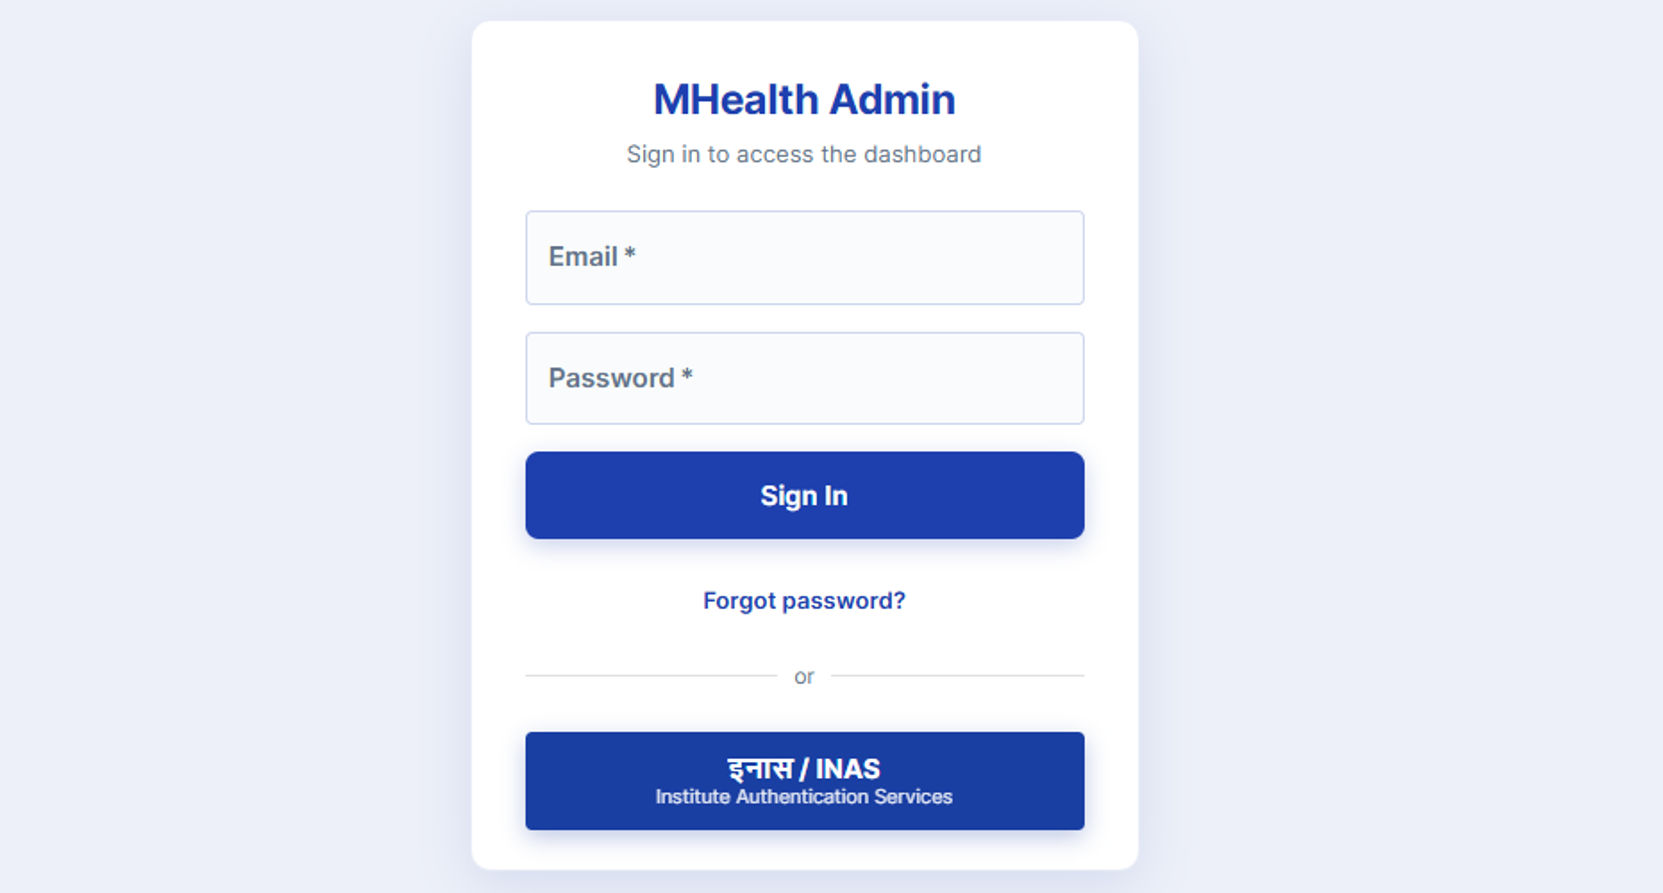
\includegraphics[width=0.75\textwidth]{Pictures/ui_login_cropped2.png}
    \caption{MHealth Admin login page. Supports email/password authentication and IITGN Institute Authentication Services (INAS) single sign-on.}
    \label{fig:ui_login}
\end{figure}

\subsubsection{Landing Page and Navigation}

After login, the counsellor is presented with the platform's landing page (Figure~\ref{fig:ui_about}), which provides navigation to three operational modules: Twilio Call Management, Call Status Dashboard, and Admin Dashboard.

\begin{figure}[h]
    \centering
    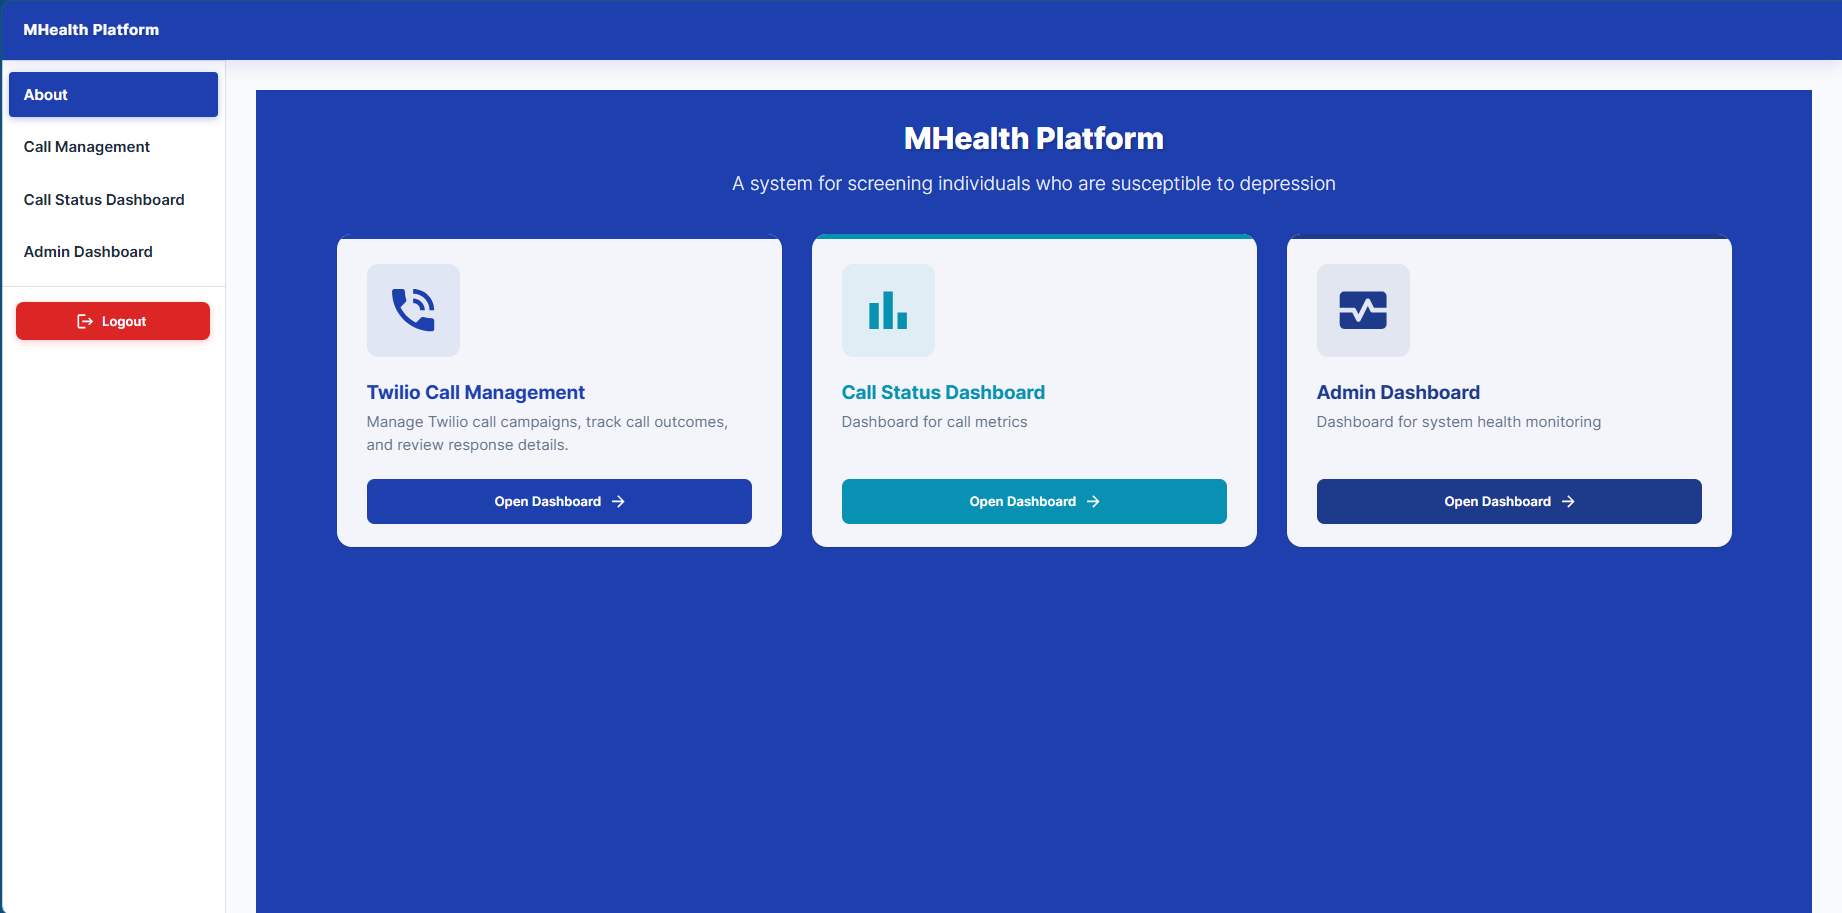
\includegraphics[width=\textwidth]{Pictures/ui_about.png}
    \caption{MHealth Platform landing page showing the three primary modules available to the counsellor after authentication.}
    \label{fig:ui_about}
\end{figure}

\subsubsection{Call Management Page}

The Call Management page (Figure~\ref{fig:ui_call_mgmt}) is the primary operational interface. It allows counsellors to:
\begin{itemize}
    \item Add individual recipients or import a list via CSV/XLSX.
    \item Select recipients and initiate Twilio calls immediately.
    \item View call history for each recipient: scheduled time, answer time, end time, overall duration, total response duration, and questions answered.
    \item Review the ML-predicted depression risk probability (e.g., \texttt{Risk Probability: 0.485} as shown in Figure~\ref{fig:ui_call_mgmt}).
    \item Play back the audio recording for each individual question response directly in the browser.
\end{itemize}

\begin{figure}[h]
    \centering
    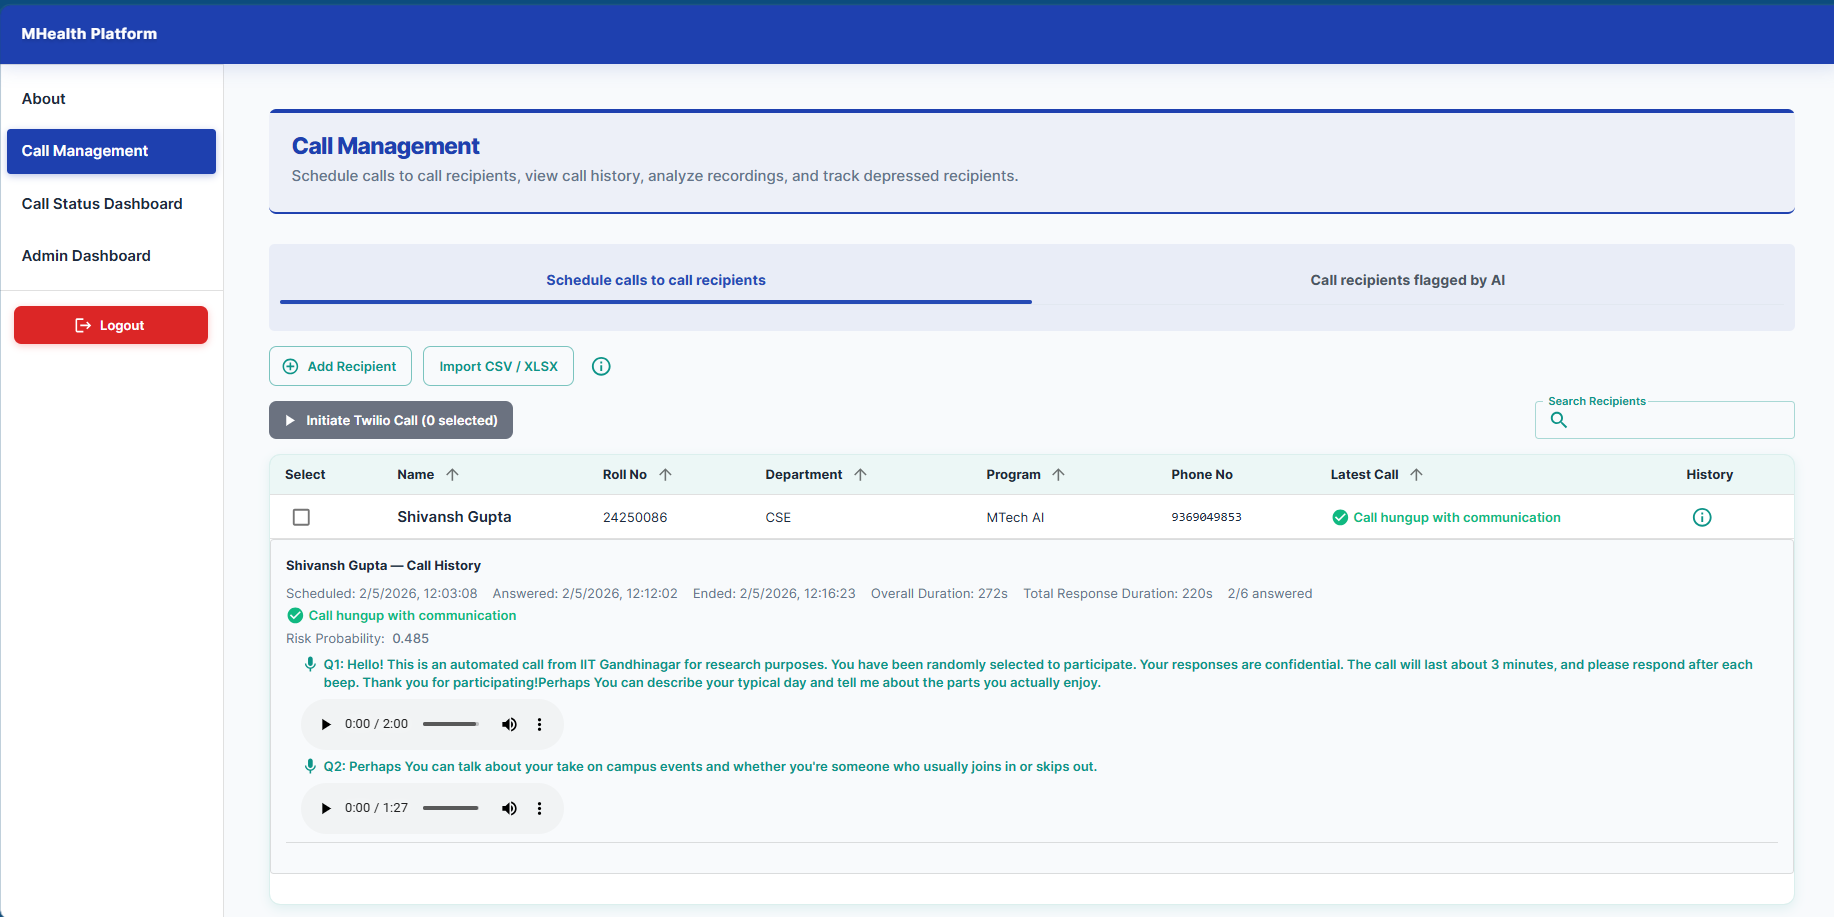
\includegraphics[width=\textwidth]{Pictures/ui_call_management.png}
    \caption{Call Management page showing a completed call for a recipient (roll no.\ 24250086). The call history panel displays the scheduled and answer times, duration, risk probability (0.485), and in-browser audio playback for each of the 6 question responses.}
    \label{fig:ui_call_mgmt}
\end{figure}

\subsubsection{AI-Flagged Recipients Tab}

Within the Call Management page, the ``Call recipients flagged by AI'' tab (Figure~\ref{fig:ui_flagged}) presents a dedicated table of students whose risk probability exceeds 0.5. This implements the human-in-the-loop design goal: the counsellor reviews this list and decides which individuals warrant follow-up. The table includes name, roll number, department, program, call timestamp, and analysis score. An export function allows the list to be downloaded for offline review.

\begin{figure}[h]
    \centering
    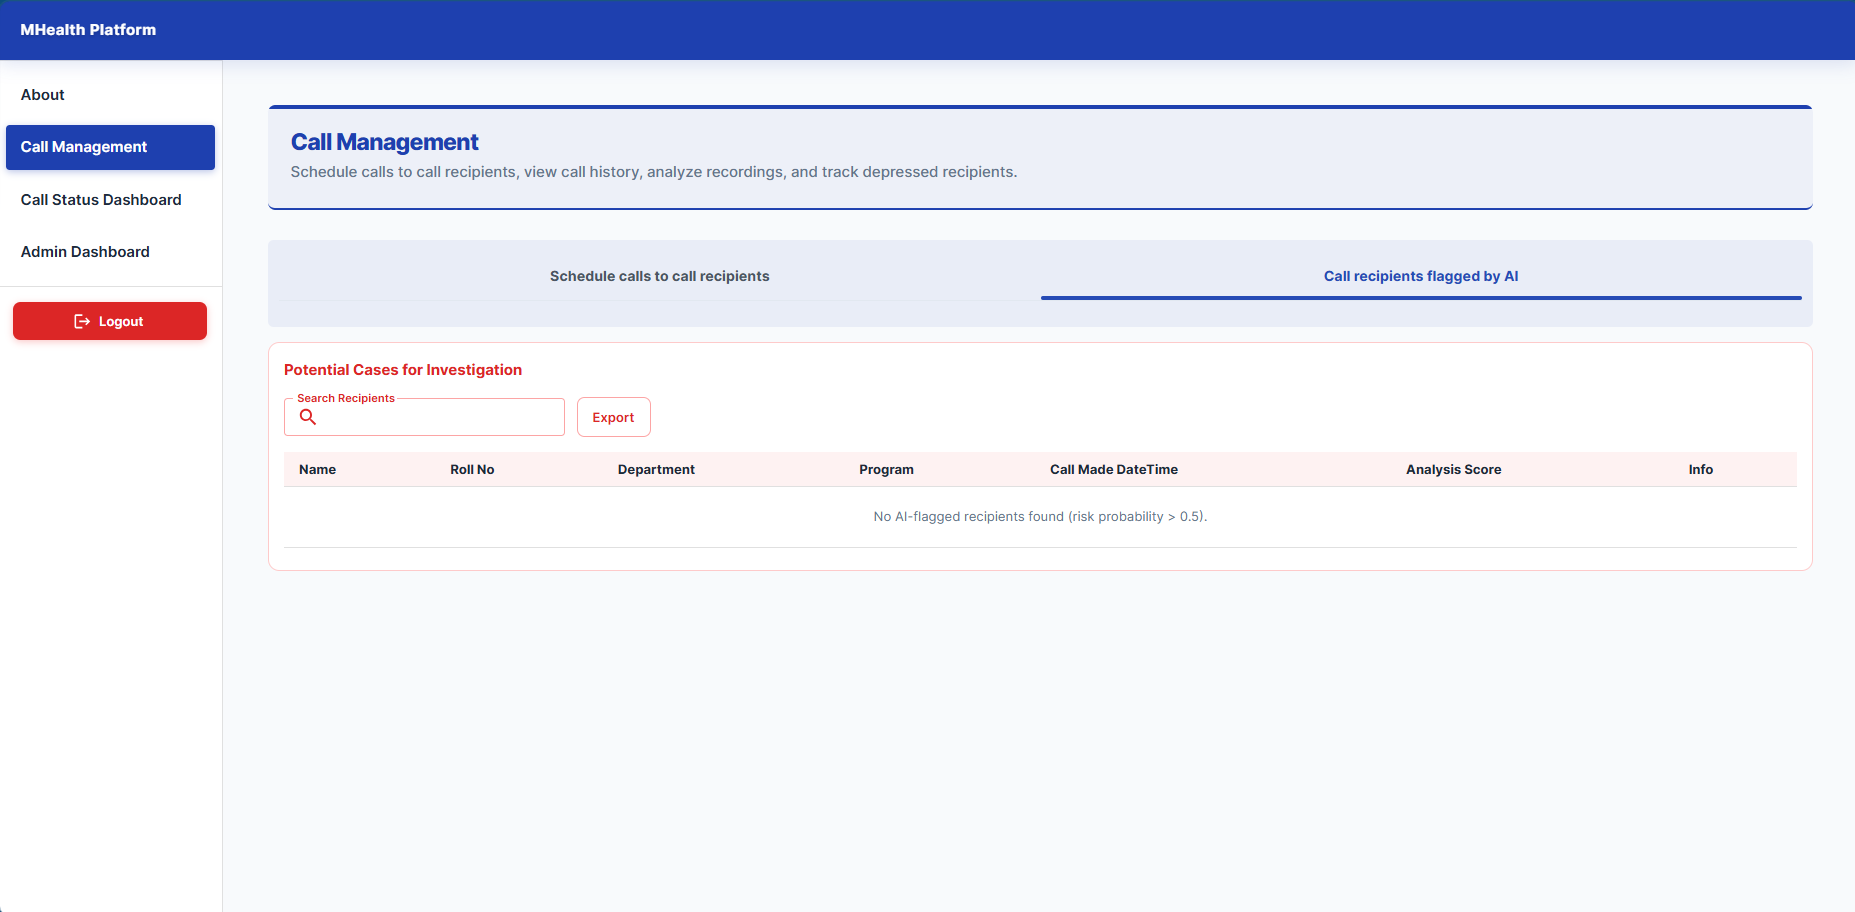
\includegraphics[width=\textwidth]{Pictures/ui_ai_flagged.png}
    \caption{``Call recipients flagged by AI'' tab showing potential cases for investigation (risk probability $> 0.5$). The counsellor reviews this list and independently decides on clinical follow-up — no automated action is taken.}
    \label{fig:ui_flagged}
\end{figure}

\subsubsection{Call Status Dashboard}

The Call Status Dashboard (Figure~\ref{fig:ui_status}) provides a real-time aggregate overview of all screening activity. It displays:
\begin{itemize}
    \item \textbf{Recipient Metrics}: Total call recipients, total predicted as depressed by the ML model, and predictions in the last 24 hours.
    \item \textbf{Call Metrics}: Total calls made and calls in the last 24 hours.
    \item \textbf{Calls by Status}: Breakdown across all call states — Scheduled, Initiated, In Progress, Not Picked, Hungup with Communication, Hungup with Short Communication, and Failed.
\end{itemize}

\begin{figure}[h]
    \centering
    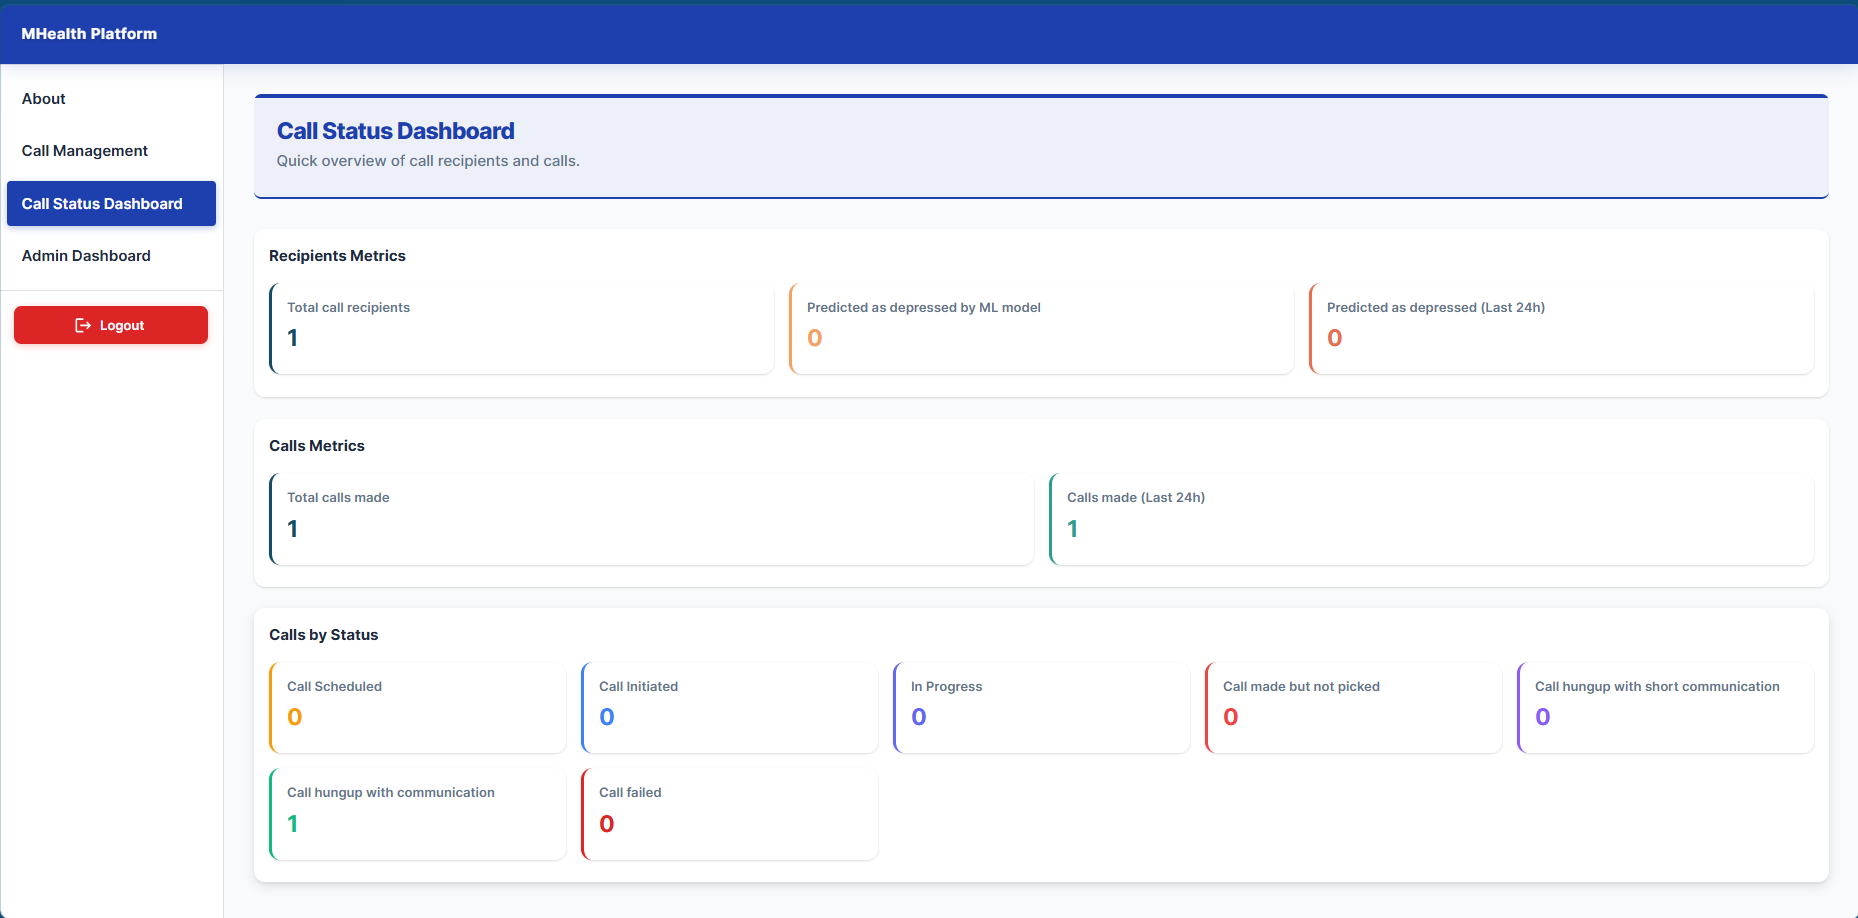
\includegraphics[width=\textwidth]{Pictures/ui_call_status.png}
    \caption{Call Status Dashboard showing recipient metrics (total recipients, ML depression predictions), call volume metrics, and a breakdown of all call outcomes by status category.}
    \label{fig:ui_status}
\end{figure}

\subsubsection{Admin Dashboard}

The Admin Dashboard (Figure~\ref{fig:ui_admin}) provides system health monitoring for the operator. It shows real-time status of all four infrastructure components — API, MinIO, Twilio SID, and Webhooks — with green checkmarks indicating operational status. It also displays the configuration overview (MinIO endpoint, bucket name, Twilio account SID, app host) and the exact webhook URLs registered with Twilio (\texttt{/voice/answer}, \texttt{/voice/status}, \texttt{/twilio}).

\begin{figure}[h]
    \centering
    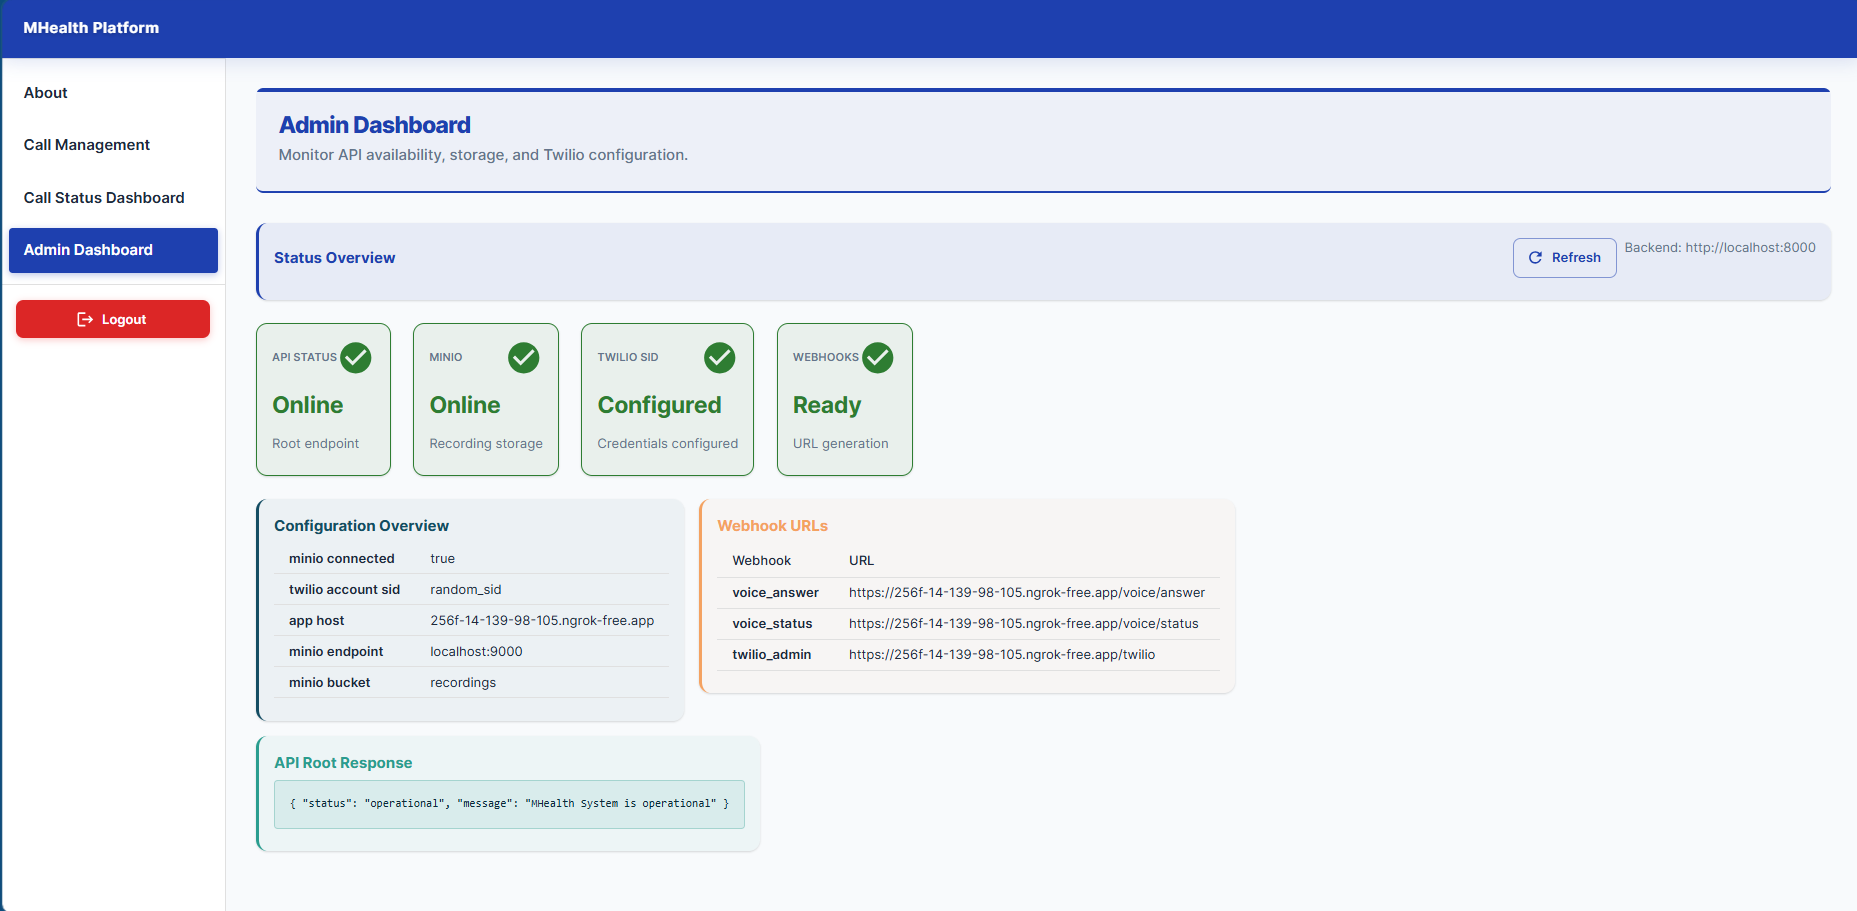
\includegraphics[width=\textwidth]{Pictures/ui_admin.png}
    \caption{Admin Dashboard showing live system health: API online, MinIO connected, Twilio SID configured, and webhooks ready. The configuration panel and active webhook URLs are displayed for operator verification.}
    \label{fig:ui_admin}
\end{figure}

\subsection{Backend API}

The main backend is a FastAPI application serving as the central orchestration layer. It exposes the following router groups:
\begin{itemize}
    \item \textbf{Auth routes} (\texttt{/auth}): Login, password reset.
    \item \textbf{ML routes} (\texttt{/api/ml}): Proxy to the ML service.
    \item \textbf{Database routes} (\texttt{/api/db}): CRUD on the main database.
    \item \textbf{Call monitoring routes} (\texttt{/api/calls}): Aggregated statistics.
    \item \textbf{Target monitoring routes} (\texttt{/api/targets}): Target-level summaries.
    \item \textbf{Counsellor routes} (\texttt{/api/counsellor}): Flagging and clinical review.
    \item \textbf{Twilio admin routes} (\texttt{/twilio}): Call initiation, history.
    \item \textbf{Twilio webhook routes} (\texttt{/voice/answer}, \texttt{/voice/respond/\{q\}}, \texttt{/voice/status}): Twilio callbacks.
\end{itemize}

\subsection{IVR Service: Twilio Voice Call Flow}

The IVR service implements the outbound call workflow using the Twilio Voice API.

\subsubsection{Call Flow}

\begin{enumerate}
    \item A counsellor triggers call initiation via the Call Management page; the backend creates a \texttt{TwilioCalls} record and queues \texttt{initiate\_twilio\_call\_task}.
    \item The Celery worker places the call using \texttt{twilio.rest.\allowbreak Client.calls.\allowbreak create()}, specifying webhook URLs for call answer and status events.
    \item When the student answers, Twilio POSTs to \texttt{/voice/answer}; the server returns TwiML for Question~0.
    \item For each question, Twilio plays the TTS prompt (Amazon Polly, \texttt{Raveena} voice, \texttt{en-IN} locale) and records the student's response via \texttt{<Record>}.
    \item After recording, Twilio POSTs to \texttt{/voice/respond/\{q\}}; the server stores the response and returns TwiML for the next question.
    \item The call ends after all 6 prompts or when total response duration reaches 180 seconds.
    \item Upon completion, two Celery tasks are queued: audio archival and ML inference.
\end{enumerate}

\subsubsection{Call Prompts}

The six open-ended prompts are designed to elicit natural, conversational speech, framed around everyday positive topics to reduce anxiety:
\begin{enumerate}
    \item Perhaps you can describe your typical day and tell me about the parts you actually enjoy.
    \item Perhaps you can talk about your take on campus events and whether you're someone who usually joins in or skips out.
    \item Describe your favourite college memory.
    \item Talk about how you and friends spend time outside class.
    \item Mention clubs or activities you are part of and what you enjoy.
    \item Share anything else on your mind about your college experience.
\end{enumerate}

All incoming Twilio webhook requests are validated against the \texttt{X-Twilio-Signature} header to prevent spoofed requests.

\subsection{ML Service}

The ML service is a dedicated FastAPI application running on port 8001. Key endpoints:
\begin{itemize}
    \item \texttt{POST /api/ml/depression}: Single-call depression prediction from audio bytes.
    \item \texttt{POST /api/ml/depression-batch}: Batch prediction for multiple files.
    \item \texttt{POST /warmup}: Pre-loads the model before traffic begins.
    \item \texttt{GET /health}: Health check with model load status.
\end{itemize}

The service uses lazy initialisation: the Random Forest model is loaded on the first prediction request, allowing the container to pass health checks before the model is ready.

\subsection{Asynchronous Task Queue: Celery and RabbitMQ}

Long-running operations are handled asynchronously by Celery workers via RabbitMQ:

\begin{table}[h]
\centering
\caption{Celery tasks in the system.}
\label{tab:celery_tasks}
\resizebox{\textwidth}{!}{%
\begin{tabular}{@{}p{6.2cm}p{8.5cm}@{}}
\toprule
\textbf{Task} & \textbf{Description} \\
\midrule
\texttt{initiate\_twilio\_call\_task}          & Places one outbound Twilio call; retries up to 3 times \\[4pt]
\texttt{archive\_call\_recordings\_task}       & Fan-out: queues one archival task per voice response \\[4pt]
\texttt{archive\_response\_recording\_task}    & Downloads one recording, uploads to MinIO, extracts duration via \texttt{ffprobe} \\[4pt]
\texttt{analyze\_call\_depression\_risk\_task} & Concatenates responses, invokes ML service, stores prediction \\[4pt]
\texttt{initiate\_calls\_for\_all\_targets}    & Defined in codebase but not active; calls are initiated manually by the counsellor via the dashboard \\
\bottomrule
\end{tabular}}
\end{table}

\subsection{Database: PostgreSQL with SQLAlchemy}

The PostgreSQL schema supports the complete counselling workflow:

\begin{table}[h]
\centering
\caption{Key database tables.}
\label{tab:db_schema}
\resizebox{\textwidth}{!}{%
\begin{tabular}{@{}p{4.8cm}p{9.5cm}@{}}
\toprule
\textbf{Table} & \textbf{Description} \\
\midrule
\texttt{TwilioTargets}           & Students enrolled in the screening programme \\
\texttt{TwilioCalls}             & Call records with depression prediction fields: risk flag, probability, level, confidence, timestamp \\
\texttt{TwilioResponses}         & Per-question responses: Twilio URL, MinIO URL, duration, question text \\
\texttt{Admins}                  & Counsellor accounts (email, hashed password) \\
\texttt{FlaggedTargets}          & Students flagged for counsellor follow-up \\
\texttt{Error\_Logs}             & System error entries \\
\texttt{Password\_Reset\_Tokens} & Time-limited tokens for password reset \\
\bottomrule
\end{tabular}}
\end{table}

\subsection{Object Storage: MinIO}

Twilio recording URLs are temporary and require authentication. To ensure long-term availability and institutional data ownership, recordings are archived to a self-hosted MinIO instance at the path:
\begin{verbatim}
twilio/{YYYY}/{MM}/{DD}/{call_sid}/{recording_filename}
\end{verbatim}

Playback is provided via presigned URLs with a 1-hour expiry. If MinIO is unavailable, the system falls back to Twilio-authenticated URLs, ensuring the ML pipeline is not blocked.

%-------------------------------------------------------------
\section{Data Flow Summary}
%-------------------------------------------------------------

The end-to-end data flow is as follows:
\begin{enumerate}
    \item Counsellor adds recipients and initiates calls from the Call Management page $\rightarrow$ DB record created $\rightarrow$ Celery queues call task.
    \item Twilio calls student $\rightarrow$ student answers $\rightarrow$ TwiML serves Question~0.
    \item Student responds (recorded) $\rightarrow$ Twilio POSTs to \texttt{/voice/respond/0}.
    \item Response saved $\rightarrow$ next prompt served; repeated for all 6 prompts.
    \item After Question~5 or 3-minute limit: call ends $\rightarrow$ archival and ML tasks queued.
    \item Archival task: recordings downloaded $\rightarrow$ uploaded to MinIO.
    \item ML task: audio concatenated $\rightarrow$ sent to ML service $\rightarrow$ prediction stored in \texttt{TwilioCalls}.
    \item Counsellor reviews Call Management page: risk probability visible, audio playback available per question (Figure~\ref{fig:ui_call_mgmt}).
    \item Students with risk probability $>$ 0.5 appear in the AI-flagged tab (Figure~\ref{fig:ui_flagged}); counsellor decides on follow-up.
\end{enumerate}

%-------------------------------------------------------------
\section{Deployment}
%-------------------------------------------------------------

The system is containerised with Docker, with separate containers for the backend, ML service, frontend, PostgreSQL, RabbitMQ, and MinIO. HTTPS is enforced at the application boundary, ensuring all Twilio webhook traffic and counsellor API calls are encrypted in transit. The Admin Dashboard (Figure~\ref{fig:ui_admin}) allows operators to verify at a glance that all infrastructure components are healthy before commencing a call campaign.

%-------------------------------------------------------------
\section{Summary}
%-------------------------------------------------------------

The proposed mHealth system is a microservices-based platform designed around seven principles: scalability, interpretability, human-in-the-loop oversight, privacy, non-intrusiveness, workflow integration, and continual improvement. Its implementation integrates Twilio IVR for automated voice collection, Celery for asynchronous processing, TSFEL-based ML inference for depression risk prediction, MinIO for secure audio storage, PostgreSQL for structured data management, and a React dashboard for counsellor interaction. The six dashboard screenshots presented in this chapter demonstrate a fully operational system deployed and tested at IIT Gandhinagar.
